\PassOptionsToPackage{unicode=true}{hyperref} % options for packages loaded elsewhere
\PassOptionsToPackage{hyphens}{url}
%
\documentclass[10pt,ignorenonframetext,serif,onlymath]{beamer}
\setbeamertemplate{caption}[numbered]
\setbeamertemplate{caption label separator}{: }
\setbeamercolor{caption name}{fg=normal text.fg}
\beamertemplatenavigationsymbolsempty
\usepackage{lmodern}
\usepackage{amssymb,amsmath}
\usepackage{ifxetex,ifluatex}
\usepackage{fixltx2e} % provides \textsubscript
\ifnum 0\ifxetex 1\fi\ifluatex 1\fi=0 % if pdftex
  \usepackage[T1]{fontenc}
  \usepackage[utf8]{inputenc}
  \usepackage{textcomp} % provides euro and other symbols
\else % if luatex or xelatex
  \usepackage{unicode-math}
  \defaultfontfeatures{Ligatures=TeX,Scale=MatchLowercase}
\fi
% use upquote if available, for straight quotes in verbatim environments
\IfFileExists{upquote.sty}{\usepackage{upquote}}{}
% use microtype if available
\IfFileExists{microtype.sty}{%
\usepackage[]{microtype}
\UseMicrotypeSet[protrusion]{basicmath} % disable protrusion for tt fonts
}{}
\IfFileExists{parskip.sty}{%
\usepackage{parskip}
}{% else
\setlength{\parindent}{0pt}
\setlength{\parskip}{6pt plus 2pt minus 1pt}
}
\usepackage{hyperref}
\hypersetup{
            pdftitle={Beamer Slides using Pandoc and Markdown},
            pdfauthor={Wai-Shing Luk},
            pdfborder={0 0 0},
            breaklinks=true}
\urlstyle{same}  % don't use monospace font for urls
\newif\ifbibliography
\usepackage{color}
\usepackage{fancyvrb}
\newcommand{\VerbBar}{|}
\newcommand{\VERB}{\Verb[commandchars=\\\{\}]}
\DefineVerbatimEnvironment{Highlighting}{Verbatim}{commandchars=\\\{\}}
% Add ',fontsize=\small' for more characters per line
\newenvironment{Shaded}{}{}
\newcommand{\AlertTok}[1]{\textcolor[rgb]{1.00,0.00,0.00}{\textbf{#1}}}
\newcommand{\AnnotationTok}[1]{\textcolor[rgb]{0.38,0.63,0.69}{\textbf{\textit{#1}}}}
\newcommand{\AttributeTok}[1]{\textcolor[rgb]{0.49,0.56,0.16}{#1}}
\newcommand{\BaseNTok}[1]{\textcolor[rgb]{0.25,0.63,0.44}{#1}}
\newcommand{\BuiltInTok}[1]{#1}
\newcommand{\CharTok}[1]{\textcolor[rgb]{0.25,0.44,0.63}{#1}}
\newcommand{\CommentTok}[1]{\textcolor[rgb]{0.38,0.63,0.69}{\textit{#1}}}
\newcommand{\CommentVarTok}[1]{\textcolor[rgb]{0.38,0.63,0.69}{\textbf{\textit{#1}}}}
\newcommand{\ConstantTok}[1]{\textcolor[rgb]{0.53,0.00,0.00}{#1}}
\newcommand{\ControlFlowTok}[1]{\textcolor[rgb]{0.00,0.44,0.13}{\textbf{#1}}}
\newcommand{\DataTypeTok}[1]{\textcolor[rgb]{0.56,0.13,0.00}{#1}}
\newcommand{\DecValTok}[1]{\textcolor[rgb]{0.25,0.63,0.44}{#1}}
\newcommand{\DocumentationTok}[1]{\textcolor[rgb]{0.73,0.13,0.13}{\textit{#1}}}
\newcommand{\ErrorTok}[1]{\textcolor[rgb]{1.00,0.00,0.00}{\textbf{#1}}}
\newcommand{\ExtensionTok}[1]{#1}
\newcommand{\FloatTok}[1]{\textcolor[rgb]{0.25,0.63,0.44}{#1}}
\newcommand{\FunctionTok}[1]{\textcolor[rgb]{0.02,0.16,0.49}{#1}}
\newcommand{\ImportTok}[1]{#1}
\newcommand{\InformationTok}[1]{\textcolor[rgb]{0.38,0.63,0.69}{\textbf{\textit{#1}}}}
\newcommand{\KeywordTok}[1]{\textcolor[rgb]{0.00,0.44,0.13}{\textbf{#1}}}
\newcommand{\NormalTok}[1]{#1}
\newcommand{\OperatorTok}[1]{\textcolor[rgb]{0.40,0.40,0.40}{#1}}
\newcommand{\OtherTok}[1]{\textcolor[rgb]{0.00,0.44,0.13}{#1}}
\newcommand{\PreprocessorTok}[1]{\textcolor[rgb]{0.74,0.48,0.00}{#1}}
\newcommand{\RegionMarkerTok}[1]{#1}
\newcommand{\SpecialCharTok}[1]{\textcolor[rgb]{0.25,0.44,0.63}{#1}}
\newcommand{\SpecialStringTok}[1]{\textcolor[rgb]{0.73,0.40,0.53}{#1}}
\newcommand{\StringTok}[1]{\textcolor[rgb]{0.25,0.44,0.63}{#1}}
\newcommand{\VariableTok}[1]{\textcolor[rgb]{0.10,0.09,0.49}{#1}}
\newcommand{\VerbatimStringTok}[1]{\textcolor[rgb]{0.25,0.44,0.63}{#1}}
\newcommand{\WarningTok}[1]{\textcolor[rgb]{0.38,0.63,0.69}{\textbf{\textit{#1}}}}
\usepackage{longtable,booktabs}
\usepackage{caption}
% These lines are needed to make table captions work with longtable:
\makeatletter
\def\fnum@table{\tablename~\thetable}
\makeatother
\usepackage{graphicx,grffile}
\makeatletter
\def\maxwidth{\ifdim\Gin@nat@width>\linewidth\linewidth\else\Gin@nat@width\fi}
\def\maxheight{\ifdim\Gin@nat@height>\textheight\textheight\else\Gin@nat@height\fi}
\makeatother
% Scale images if necessary, so that they will not overflow the page
% margins by default, and it is still possible to overwrite the defaults
% using explicit options in \includegraphics[width, height, ...]{}
\setkeys{Gin}{width=\maxwidth,height=\maxheight,keepaspectratio}
% Prevent slide breaks in the middle of a paragraph:
\widowpenalties 1 10000
\raggedbottom
\setbeamertemplate{part page}{
\centering
\begin{beamercolorbox}[sep=16pt,center]{part title}
  \usebeamerfont{part title}\insertpart\par
\end{beamercolorbox}
}
\setbeamertemplate{section page}{
\centering
\begin{beamercolorbox}[sep=12pt,center]{part title}
  \usebeamerfont{section title}\insertsection\par
\end{beamercolorbox}
}
\setbeamertemplate{subsection page}{
\centering
\begin{beamercolorbox}[sep=8pt,center]{part title}
  \usebeamerfont{subsection title}\insertsubsection\par
\end{beamercolorbox}
}
\AtBeginPart{
  \frame{\partpage}
}
\AtBeginSection{
  \ifbibliography
  \else
    \frame{\sectionpage}
  \fi
}
\AtBeginSubsection{
  \frame{\subsectionpage}
}
\setlength{\emergencystretch}{3em}  % prevent overfull lines
\providecommand{\tightlist}{%
  \setlength{\itemsep}{0pt}\setlength{\parskip}{0pt}}
\setcounter{secnumdepth}{0}

% set default figure placement to htbp
\makeatletter
\def\fps@figure{htbp}
\makeatother

\usetheme{default}
\ifxetex \usepackage[UTF8]{ctex} \fi
\usepackage[footnotesize]{subfigure}
\usepackage{tikz,pgf,pgfplots}
\usetikzlibrary{arrows}
\definecolor{qqqqff}{rgb}{0.,0.,1.}
\newcommand{\columnsbegin}{\begin{columns}}
\newcommand{\columnsend}{\end{columns}}
\newcommand{\col}[1]{\column{#1}}
\pgfdeclareimage[height=0.5cm]{fudan-logo}{fudan-logo.jpg}
\logo{\pgfuseimage{fudan-logo}}

\title{Beamer Slides using Pandoc and Markdown}
\author{Wai-Shing Luk}
\providecommand{\institute}[1]{}
\institute{Fudan University}
\date{\today}

\begin{document}
\frame{\titlepage}

\begin{frame}{Introduction}
\protect\hypertarget{sec:intro}{}

\begin{block}{Why Markup Language?}

\begin{itemize}
\tightlist
\item
  Separate “content” with “style”.
\end{itemize}

\end{block}

\begin{block}{Why Pandoc and Beamer?}

\begin{itemize}
\tightlist
\item
  For professional presentation.
\item
  Tikz diagrams.
\end{itemize}

\end{block}

\end{frame}

\begin{frame}[fragile]{A simple example \texttt{intro.md}}
\protect\hypertarget{sec:a-simple-example-intro.md}{}

\begin{Shaded}
\begin{Highlighting}[]
\NormalTok{---}
\NormalTok{title: Beamer Slides using Pandoc and Markdown}
\NormalTok{author: Wai-Shing Luk}
\NormalTok{bibliography: papers.bib}
\NormalTok{...}

\FunctionTok{## Introduction \{#sec:intro\}}

\FunctionTok{### Why Markup Language?}

\NormalTok{- }\FloatTok{  Separate "content" with "style".}

\FunctionTok{### Why Beamer?}

\NormalTok{- }\FloatTok{  For professional presentation.}
\FloatTok{-   Tikz diagrams.}
\end{Highlighting}
\end{Shaded}

\end{frame}

\begin{frame}[fragile]{\texttt{pandoc}}
\protect\hypertarget{sec:pandoc}{}

Pandoc is a Haskell library for converting from one markup format to
another\footnote<.->{This is a footnote.}, and a command-line tool that
uses this library. It can read Markdown and write \LaTeX~or Beamer.

To compile:

\begin{Shaded}
\begin{Highlighting}[]
\NormalTok{$ }\ExtensionTok{pandoc}\NormalTok{ -s -t beamer beamer.yaml intro.md -o intro.tex}
\end{Highlighting}
\end{Shaded}

or directly to a pdf file:

\begin{Shaded}
\begin{Highlighting}[]
\NormalTok{$ }\ExtensionTok{pandoc}\NormalTok{ -t beamer beamer.yaml intro.md -o intro.pdf}
\end{Highlighting}
\end{Shaded}

\end{frame}

\begin{frame}[fragile]{A simple header \texttt{beamer.yaml}}
\protect\hypertarget{sec:a-simple-header-beamer.yaml}{}

\scriptsize

\begin{Shaded}
\begin{Highlighting}[]
\OtherTok{---}
\FunctionTok{fontsize:}\AttributeTok{ 10pt}
\FunctionTok{classoption:}
  \KeywordTok{-}\NormalTok{ serif,onlymath}
\FunctionTok{institute:}\AttributeTok{ Fudan University}
\FunctionTok{date:}\AttributeTok{ \textbackslash{}today}
\FunctionTok{header-includes:}
  \KeywordTok{-}\NormalTok{ \textbackslash{}usetheme}\KeywordTok{\{}\NormalTok{default}\KeywordTok{\}}
  \KeywordTok{-}\NormalTok{ \textbackslash{}usepackage}\KeywordTok{[}\NormalTok{footnotesize}\KeywordTok{]\{}\NormalTok{subfigure}\KeywordTok{\}}
  \KeywordTok{-}\NormalTok{ \textbackslash{}usepackage}\KeywordTok{\{}\NormalTok{tikz,pgf,pgfplots}\KeywordTok{\}}
  \KeywordTok{-}\NormalTok{ \textbackslash{}usetikzlibrary}\KeywordTok{\{}\NormalTok{arrows}\KeywordTok{\}}
  \KeywordTok{-}\NormalTok{ \textbackslash{}definecolor}\KeywordTok{\{}\NormalTok{qqqqff}\KeywordTok{\}\{}\NormalTok{rgb}\KeywordTok{\}\{}\NormalTok{0.,0.,1.}\KeywordTok{\}}
  \KeywordTok{-}\NormalTok{ \textbackslash{}newcommand}\KeywordTok{\{}\NormalTok{\textbackslash{}columnsbegin}\KeywordTok{\}\{}\NormalTok{\textbackslash{}begin\{columns}\KeywordTok{\}}\NormalTok{\}}
  \KeywordTok{-}\NormalTok{ \textbackslash{}newcommand}\KeywordTok{\{}\NormalTok{\textbackslash{}columnsend}\KeywordTok{\}\{}\NormalTok{\textbackslash{}end\{columns}\KeywordTok{\}}\NormalTok{\}}
  \KeywordTok{-}\NormalTok{ \textbackslash{}newcommand}\KeywordTok{\{}\NormalTok{\textbackslash{}col}\KeywordTok{\}[}\NormalTok{1}\KeywordTok{]\{}\NormalTok{\textbackslash{}column\{}\CommentTok{#1\}\}}
\NormalTok{  - \textbackslash{}pgfdeclareimage[height=0.5cm]\{fudan-logo}\KeywordTok{\}\{}\NormalTok{fudan-logo.jpg}\KeywordTok{\}}
  \KeywordTok{-}\NormalTok{ \textbackslash{}logo}\KeywordTok{\{}\NormalTok{\textbackslash{}pgfuseimage\{fudan-logo}\KeywordTok{\}}\NormalTok{\}}
\CommentTok{...}
\end{Highlighting}
\end{Shaded}

\end{frame}

\begin{frame}[fragile]{Render Mathematical Equations using LaTeX}
\protect\hypertarget{sec:render-mathematical-equations-using-latex}{}

\begin{columns}

\column{0.5\textwidth}

\scriptsize

\begin{Shaded}
\begin{Highlighting}[]

\NormalTok{Consider the following problem:}

\SpecialStringTok{$$}\SpecialCharTok{\textbackslash{}begin}\SpecialStringTok{\{array\}\{ll\}}
\SpecialStringTok{  }\SpecialCharTok{\textbackslash{}text}\NormalTok{\{minimize\}}\SpecialStringTok{    & f_0(x), }\SpecialCharTok{\textbackslash{}\textbackslash{}}
\SpecialStringTok{  }\SpecialCharTok{\textbackslash{}text}\NormalTok{\{subject to\}}\SpecialStringTok{  & F(x) }\SpecialCharTok{\textbackslash{}succeq}\SpecialStringTok{ 0,}
\SpecialCharTok{\textbackslash{}end}\SpecialStringTok{\{array\}$$}\NormalTok{ \{#eq:semidef\}}

\NormalTok{- }\SpecialStringTok{$F(x)$}\NormalTok{: a matrix-valued function}
\NormalTok{- }\SpecialStringTok{$A }\SpecialCharTok{\textbackslash{}succeq}\SpecialStringTok{ 0$}\NormalTok{ denotes }\SpecialStringTok{$A$}\NormalTok{ is}
\NormalTok{  positive semidefinite.}
\end{Highlighting}
\end{Shaded}

\column{0.5\textwidth}

Consider the following problem:

\protect\hypertarget{eq:semidef}{}{\[\begin{array}{ll}
  \text{minimize}    & f_0(x), \\
  \text{subject to}  & F(x) \succeq 0,
\end{array}\qquad(1)\]}

\begin{itemize}
\tightlist
\item
  \(F(x)\): a matrix-valued function
\item
  \(A \succeq 0\) denotes \(A\) is positive semidefinite.
\end{itemize}

\end{columns}

\end{frame}

\begin{frame}[fragile]{How to make a two-column slide}
\protect\hypertarget{sec:how-to-make-a-two-column-slide}{}

\begin{Shaded}
\begin{Highlighting}[]

\NormalTok{\textbackslash{}columnsbegin}

\NormalTok{\textbackslash{}col\{0.5\textbackslash{}textwidth\}}

\NormalTok{  Left-hand side}

\NormalTok{\textbackslash{}col\{0.5\textbackslash{}textwidth\}}

\NormalTok{  Right-hand side}

\NormalTok{\textbackslash{}columnsend}
\end{Highlighting}
\end{Shaded}

\end{frame}

\begin{frame}[fragile]{Figures}
\protect\hypertarget{sec:figures}{}

An image occurring by itself in a paragraph will be rendered as a figure
with a caption.

\begin{figure}
\hypertarget{fig:figure0}{%
\centering
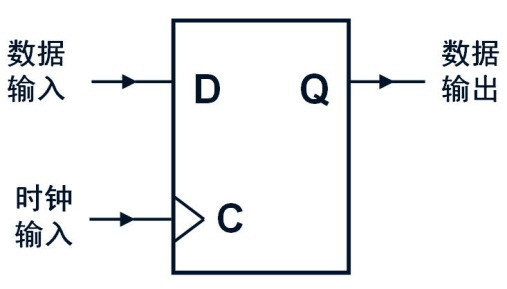
\includegraphics{media/image2.jpeg}
\caption{This is the caption}\label{fig:figure0}
}
\end{figure}

(source)

\begin{Shaded}
\begin{Highlighting}[]
\AlertTok{![This is the caption](media/image2.jpeg)}\NormalTok{\{#fig:figure0\}}
\end{Highlighting}
\end{Shaded}

\end{frame}

\begin{frame}[fragile]{Figures (cont’d)}
\protect\hypertarget{sec:figures-contd}{}

If you just want a regular inline image, just make sure it is not the
only thing in the paragraph. One way to do this is to insert a
nonbreaking space after the image:

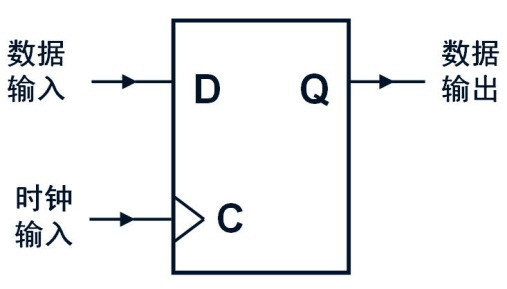
\includegraphics{media/image2.jpeg}\\

(source)

\begin{Shaded}
\begin{Highlighting}[]
\AlertTok{![No caption](media/image2.jpeg)}\NormalTok{\textbackslash{}}
\end{Highlighting}
\end{Shaded}

\end{frame}

\begin{frame}[fragile]{Render Diagrams using Tikz}
\protect\hypertarget{sec:render-diagrams-using-tikz}{}

\begin{columns}

\column{0.4\textwidth}
\scriptsize

\begin{Shaded}
\begin{Highlighting}[]

\KeywordTok{\textbackslash{}begin}\NormalTok{\{}\ExtensionTok{figure}\NormalTok{\}[hp]}
\FunctionTok{\textbackslash{}centering}
\FunctionTok{\textbackslash{}input}\NormalTok{\{pole2polar.tikz\}}
\FunctionTok{\textbackslash{}caption}\NormalTok{\{Example of constructing}
\NormalTok{    the polar of a point\}}\CommentTok{%}
\KeywordTok{\textbackslash{}label}\NormalTok{\{}\ExtensionTok{fig:pole2polar}\NormalTok{\}}
\KeywordTok{\textbackslash{}end}\NormalTok{\{}\ExtensionTok{figure}\NormalTok{\}}
\end{Highlighting}
\end{Shaded}

\column{0.6\textwidth}

\begin{figure}[hp]
\centering
\definecolor{uuuuuu}{rgb}{0.26666666666666666,0.26666666666666666,0.26666666666666666}
\definecolor{ffqqqq}{rgb}{1.,0.,0.}
\definecolor{qqqqff}{rgb}{0.,0.,1.}
\definecolor{cqcqcq}{rgb}{0.7529411764705882,0.7529411764705882,0.7529411764705882}
\begin{tikzpicture}[scale=0.5,line cap=round,line join=round,>=triangle 45,x=1.0cm,y=1.0cm]
\draw [color=cqcqcq,, xstep=1.0cm,ystep=1.0cm] (-4.3,-6.2) grid (12.42,6.3);
\clip(-4.3,-6.2) rectangle (12.42,6.3);
\onslide<7->{
  \draw [rotate around={0.:(2.5,0.5)}] (2.5,0.5) ellipse (3.1024184114977142cm and 2.533114025595111cm);
}
\onslide<9->{
  \draw [domain=-4.3:12.42] plot(\x,{(-30.--3.*\x)/-7.});
}
\onslide<11->{
  \draw [domain=-4.3:12.42] plot(\x,{(--10.-1.*\x)/-10.});
}
\onslide<13->{
  \draw [domain=-4.3:12.42] plot(\x,{(-14.306522167487685--2.7190541871921186*\x)/-0.6334581280788179});
}
\onslide<14->{
  \draw [domain=-4.3:12.42] plot(\x,{(-3.--4.*\x)/3.});
}
\onslide<16->{
  \draw [domain=-4.3:12.42] plot(\x,{(--4.736-3.256*\x)/-4.736});
}
\onslide<17->{
  \draw [domain=-4.3:12.42] plot(\x,{(-17.497536945812808--3.4630541871921183*\x)/-2.3694581280788176});
}
\onslide<19->{
  \draw [color=ffqqqq,domain=-4.3:12.42] plot(\x,{(--10.85435667986003-2.9074169678196515*\x)/-0.2907416967819647});
}
\begin{scriptsize}
\onslide<3->{
  \draw [fill=qqqqff] (3.,3.) circle (2.5pt);
}
\onslide<3->{
  \draw[color=qqqqff] (3.14,3.36) node {$B$};
}
\onslide<6->{
  \draw [fill=qqqqff] (0.,-1.) circle (2.5pt);
}
\onslide<6->{
  \draw[color=qqqqff] (0.14,-0.64) node {$E$};
}
\onslide<7->{
  \draw[color=black] (1.,2.42) node {$c$};
}
\onslide<8->{
  \draw [fill=ffqqqq] (10.,0.) circle (2.5pt);
}
\onslide<8->{
  \draw[color=ffqqqq] (10.14,0.36) node {$F$};
}
\onslide<9->{
  \draw[color=black] (-4.14,5.9) node {$f$};
}
\onslide<10->{
  \draw [fill=uuuuuu] (4.736,2.256) circle (1.5pt);
}
\onslide<10->{
  \draw[color=uuuuuu] (4.88,2.54) node {$G$};
}
\onslide<11->{
  \draw[color=black] (12.18,0.08) node {$g$};
}
\onslide<12->{
  \draw [fill=uuuuuu] (5.369458128078818,-0.4630541871921182) circle (1.5pt);
}
\onslide<12->{
  \draw[color=uuuuuu] (5.5,-0.18) node {$H$};
}
\onslide<13->{
  \draw[color=black] (4.04,6.16) node {$h$};
}
\onslide<14->{
  \draw[color=black] (5.04,6.16) node {$i$};
}
\onslide<15->{
  \draw [fill=uuuuuu] (4.192307692307692,4.5897435897435885) circle (1.5pt);
}
\onslide<15->{
  \draw[color=uuuuuu] (4.34,4.86) node {$I$};
}
\onslide<16->{
  \draw[color=black] (-4.14,-3.48) node {$j$};
}
\onslide<17->{
  \draw[color=black] (8.9,-5.94) node {$k$};
}
\onslide<18->{
  \draw [fill=uuuuuu] (3.901565995525727,1.6823266219239372) circle (1.5pt);
}
\onslide<18->{
  \draw[color=uuuuuu] (4.04,1.96) node {$J$};
}
\onslide<19->{
  \draw[color=ffqqqq] (4.08,6.16) node {$l$};
}
\end{scriptsize}
\end{tikzpicture}

\caption{Example of constructing
    the polar of a point}%
\label{fig:pole2polar}
\end{figure}

\end{columns}

\end{frame}

\begin{frame}[fragile]{Table}
\protect\hypertarget{sec:table}{}

Simple tables can be generated using Markdown.

\scriptsize

\begin{columns}

\column{0.5\textwidth}

\begin{Shaded}
\begin{Highlighting}[]

\NormalTok{| Costs        |   28nm     |    20nm     |}
\NormalTok{|--------------|------------|-------------|}
\NormalTok{| Fab Costs    | 3B         |  4B - 7B    |}
\NormalTok{| Process R&D  | 1.2B       | 2.1B - 3B   |}
\NormalTok{| Mask Costs   | 2M - 3M    | 5M - 8M     |}
\NormalTok{| Design Costs | 50M - 90M  | 120M - 500M |}

\NormalTok{: Fab, process, mask, and design}
\NormalTok{  costs \{#tbl:fab\}}
\end{Highlighting}
\end{Shaded}

\column{0.5\textwidth}

\hypertarget{tbl:fab}{}
\begin{longtable}[]{@{}lll@{}}
\caption{Fab, process, mask, and design costs}\tabularnewline
\toprule
Costs & 28nm & 20nm\tabularnewline
\midrule
\endfirsthead
\toprule
Costs & 28nm & 20nm\tabularnewline
\midrule
\endhead
Fab Costs & 3B & 4B - 7B\tabularnewline
Process R\&D & 1.2B & 2.1B - 3B\tabularnewline
Mask Costs & 2M - 3M & 5M - 8M\tabularnewline
Design Costs & 50M - 90M & 120M - 500M\tabularnewline
\bottomrule
\end{longtable}

\end{columns}

\end{frame}

\begin{frame}[fragile]{\texttt{pandoc-crossref} filter}
\protect\hypertarget{sec:pandoc-crossref-filter}{}

With this filter, you can cross-reference figures (see Fig.~1 and Fig.
\ref{fig:pole2polar}), display equations (see Eq.~1), tables (see
Table~1) and sections (§~1.1, 1.3)

There is also support for code blocks, for example, Listing~1, 2.

To compile:

\begin{Shaded}
\begin{Highlighting}[]
\NormalTok{$ }\ExtensionTok{pandoc}\NormalTok{ -F pandoc-crossref -t beamer beamer.yaml \textbackslash{}}
\NormalTok{  crossref.yaml beamer.md -o intro.pdf}
\end{Highlighting}
\end{Shaded}

\end{frame}

\begin{frame}[fragile]{A sample \texttt{crossref.yaml}}
\protect\hypertarget{sec:a-sample-crossref.yaml}{}

\scriptsize

\begin{Shaded}
\begin{Highlighting}[]
\OtherTok{---}
\FunctionTok{cref:}\AttributeTok{ True}
\FunctionTok{codeBlockCaptions:}\AttributeTok{ True}
\FunctionTok{lofTitle:}\AttributeTok{ }\StringTok{"## List of Figures"}
\FunctionTok{lotTitle:}\AttributeTok{ }\StringTok{"## List of Tables"}
\FunctionTok{autoSectionLabels:}\AttributeTok{ True}
\FunctionTok{figureTemplate:}\AttributeTok{ $$t$$}
\FunctionTok{tableTemplate:}\AttributeTok{ $$t$$}
\FunctionTok{figPrefix:}
  \KeywordTok{-} \StringTok{"Fig."}
\FunctionTok{eqnPrefix:}
  \KeywordTok{-} \StringTok{"Eq."}
\FunctionTok{tblPrefix:}
  \KeywordTok{-} \StringTok{"Table"}
\FunctionTok{lstPrefix:}
  \KeywordTok{-} \StringTok{"Listing"}
\FunctionTok{secPrefix:}
  \KeywordTok{-} \StringTok{"§"}
\CommentTok{...}
\end{Highlighting}
\end{Shaded}

\end{frame}

\begin{frame}[fragile]{Code blocks}
\protect\hypertarget{sec:code-blocks}{}

There are a couple options for code block labels. Those work only if
code block id starts with \texttt{lst:}, e.g. \texttt{\{\#lst:label\}}

\end{frame}

\begin{frame}[fragile]{\texttt{caption} attribute}
\protect\hypertarget{sec:caption-attr}{}

\texttt{caption} attribute will be treated as code block caption. If
code block has both id and \texttt{caption} attributes, it will be
treated as numbered code block.

\leavevmode\hypertarget{lst:captionAttr}{}%
Listing 1: Listing caption A

\begin{Shaded}
\begin{Highlighting}[]
\OtherTok{main ::} \DataTypeTok{IO}\NormalTok{ ()}
\NormalTok{main }\FunctionTok{=}\NormalTok{ putStrLn }\StringTok{"Hello World!"}
\end{Highlighting}
\end{Shaded}

(source)

\begin{Shaded}
\begin{Highlighting}[]
\NormalTok{\{#lst:captionAttr .haskell caption="Listing caption A"\}}
\end{Highlighting}
\end{Shaded}

\end{frame}

\begin{frame}[fragile]{Table-style captions}
\protect\hypertarget{sec:table-capts}{}

Enabled with \texttt{codeBlockCaptions} metadata option. If code block
is immediately adjacent to paragraph, starting with \texttt{Listing:} or
\texttt{:}, said paragraph will be treated as code block caption.

\leavevmode\hypertarget{lst:tableCaption}{}%
Listing 2: Listing caption B

\begin{Shaded}
\begin{Highlighting}[]
\OtherTok{main ::} \DataTypeTok{IO}\NormalTok{ ()}
\NormalTok{main }\FunctionTok{=}\NormalTok{ putStrLn }\StringTok{"Hello World!"}
\end{Highlighting}
\end{Shaded}

\end{frame}

\begin{frame}[fragile]{Bibliography}
\protect\hypertarget{sec:bibliography}{}

\scriptsize

\begin{columns}

\column{0.5\textwidth}

\begin{Shaded}
\begin{Highlighting}[]

\NormalTok{- }\FloatTok{See @Aalst-etal_2004, or}
\FloatTok{- See [@Baldi-etal_2008;@Canfora-Cerulo_2005a].}
\end{Highlighting}
\end{Shaded}

\column{0.5\textwidth}

\begin{itemize}
\tightlist
\item
  See Aalst, Weijters, and Maruster (2004), or
\item
  See (Baldi et al. 2008; Canfora and Cerulo 2005).
\end{itemize}

\end{columns}

To compile:

\begin{Shaded}
\begin{Highlighting}[]
\NormalTok{$ }\ExtensionTok{pandoc}\NormalTok{ -F pandoc-crossref -F pandoc-citeproc -t beamer \textbackslash{}}
\NormalTok{  beamer.yaml crossref.yaml beamer.md -o intro.pdf}
\end{Highlighting}
\end{Shaded}

\end{frame}

\begin{frame}{References}
\protect\hypertarget{sec:references}{}

\hypertarget{refs}{}
\leavevmode\hypertarget{ref-Aalst-etal_2004}{}%
Aalst, W. van der, T. Weijters, and L. Maruster. 2004. “Workflow Mining:
Discovering Process Models from Event Logs.” \emph{IEEE Transactions on
Knowledge and Data Engineering} 16 (9). Los Alamitos, CA, USA: IEEE
Computer Society:1128–42. \url{https://doi.org/10.1109/TKDE.2004.47}.

\leavevmode\hypertarget{ref-Baldi-etal_2008}{}%
Baldi, Pierre F, Cristina V Lopes, Erik J Linstead, and Sushil K
Bajracharya. 2008. “A Theory of Aspects as Latent Topics.” In \emph{ACM
Sigplan Notices}, 43:543–62. 10. ACM.
\url{https://doi.org/10.1145/1449955.1449807}.

\leavevmode\hypertarget{ref-Canfora-Cerulo_2005a}{}%
Canfora, G., and L. Cerulo. 2005. “Impact Analysis by Mining Software
and Change Request Repositories.” In \emph{11th Ieee International
Software Metrics Symposium (Metrics’05)}, 29. Como, Italy: IEEE.
\url{https://doi.org/10.1109/METRICS.2005.28}.

\end{frame}

\end{document}
